\documentclass[
    12pt,
    ngerman,
    fleqn,
    parskip=half,
    DIV=15, BCOR=2cm, headinclude,
]{scrbook}

%\includeonly{40-Implementierung}

\usepackage{header}

\def\table{\def\figurename{Tabelle}\figure}
\let\endtable\endfigure 

\usepackage{csquotes}
\usepackage{booktabs}
\usepackage{algpseudocode}
\usepackage{placeins}

\usepackage{float}
\newfloat{algorithm}{tbhp}{loa}[chapter]
\floatname{algorithm}{Algorithmus}

\usepackage{tikz}
\usepackage{pgfplots}
\pgfplotsset{
    compat=1.9,
    width=0.8\linewidth,
    xticklabel style={/pgf/number format/use comma},
    yticklabel style={/pgf/number format/use comma},
}
\usepgfplotslibrary{external}
\tikzexternalize[mode=list and make]
\tikzsetexternalprefix{_build/Abbildung-}

\pgfplotsset{
    colormap={whiteblack}{gray=(0.95) gray=(0)},
    max space between ticks=50pt,
}


\hypersetup{
    pdftitle={%
        Konstruktion eines Wirbelbettes auf Gas- und Wasserbasis
    }
}

\usepackage{datetime}

\newcommand\bootstrapsamples{N_\text P}
\newcommand\gausswidth{\sigma}
\newcommand\initialrandomwidth{\tilde \Delta}
\newcommand\iterations{M}
\newcommand\iterationsbetween{M_\text{Zw}}
\newcommand\margin{\Delta}
\newcommand\mass{\mu}
\newcommand\preiterations{M'}
\newcommand\rounds{\bar n}
\newcommand\timesites{N}
\newcommand\timestep{a}



\subject{Bachelorarbeit in Physikingenieurwesen}
\title{%
    Konstruktion eines Wirbelbettes auf Gas- und Wasserbasis
}
%\subtitle{}
\author{
    Christoph Hansen \\ \small{\href{mailto:ch@chrstophhansen.eu}{ch@christophhansen.eu}}
}
\publishers{%
	Angefertigt im Institut für Materialwissenschaft im Weltraum am DLR, vorgelegt dem Fachbereich 10 der Fachhochschule Aachen
}
\date{April 2015}

\uppertitleback{%
    1. Gutachter: Prof. Dr. Michael Stellberg \\
    2. Gutachter: Dr. Matthias Sperl
}

\lowertitleback{%
}

\begin{document}

\maketitle



\tableofcontents

\newpage

\chapter{Einleitung}


\section{Einführung}

Bei fast allen Stoffen muss die Stofftemperatur ändern, damit sie in einen anderen Aggregatzustand wechseln. Bei granularen Medien ist das nicht nötig, stattdessen wird eine Säule des Mediums mittles unterschiedlich hoher Luftdurchsätze zu den verschiedenen Aggregatzustänge angeregt. \\
Da man bisher kein tiefgehendes Verständnis darüber hat welche Parameter sich wie auf die Entstehung der einzelnen Aggregatzustände auswirken, soll dies im Rahmen einer Doktorarbeit untersucht werden. \\
Ausgang war ein Aufbau eines Wirbelbettes, das allerdings nur begrenzt nutzbar war und sich auf Grund verschiedener Unzulänglichkeiten, nur für qualitative Messungen nutzen lies. \\
\hfill \\
Diese Arbeit behandelt die Neukonzeption des bestehenden Wirbelbettes am Deutschen Zentrum für Luft- und Raumfahrt, Institut für Materialphysik im Weltraum. Dabei geht es vor allen Dingen darum mit welchen konstruktiven Lösungen die Mängel des bisherigen Wirbelbettes behoben wurden. Weiterhin werden Testmessungen gemacht, um die Funktion des Wirbelbettes nachzuweisen.



\section{Grundlegende Begrifflichkeiten}

\subsection{Granulare Medien}

Unter Granulat versteht man ein Medium, das aus einzelnen harten Körnern besteht, die jeweils den Gesetzen der Newtonschen Mechanik unterworfen sind. Weiterhin haben die Körner eine Mindestgröße von $\SI{10}{\micro\meter}$, dabei spielt die Form der Oberfläche keine Rolle. Dies folgt aus der Forderung, das Schwingungen die Körner nicht mehr als ganzes anregen können sollen. \\
Ein weiteres Charakteristikum von Granulaten ist die Dissipertivität. Das heißt, dass die hauptsächlich kinetische Energie der Körner fast komplett in Wärmeenergie umgewandelt werden kann. Hier gilt die Energieerhaltung der klassischen Mechanik nicht. \\
Daraus ergibt sich als weiteres Merkmal granularer Medien die Sedimentation. Das bedeutet, das sich kleinere Partikel zwischen größeren bewegen können und so eine höhere Packungsdichte erreicht wird. \\
\hfill \\ 
Wie bei Molekülen gibt es auch bei granularen Medien ein dynamisches Verhalten. Dieses kann man hervorrufen, indem man mittels Schwingungen, also Vibration, auf das Granulat einwirkt. Man erhält dann ein schwingungsfluidiertes Granulat, in dem die Bewegung der Teilchen mit der Brownschen Molekularbewegung vergleichbar ist. \\
Die unterschiedlichen Energiezustände des Granulats werden gerne mit den Aggregatzuständen molekularer Stoffe verglichen:


\begin{center}
\begin{figure}[h]
	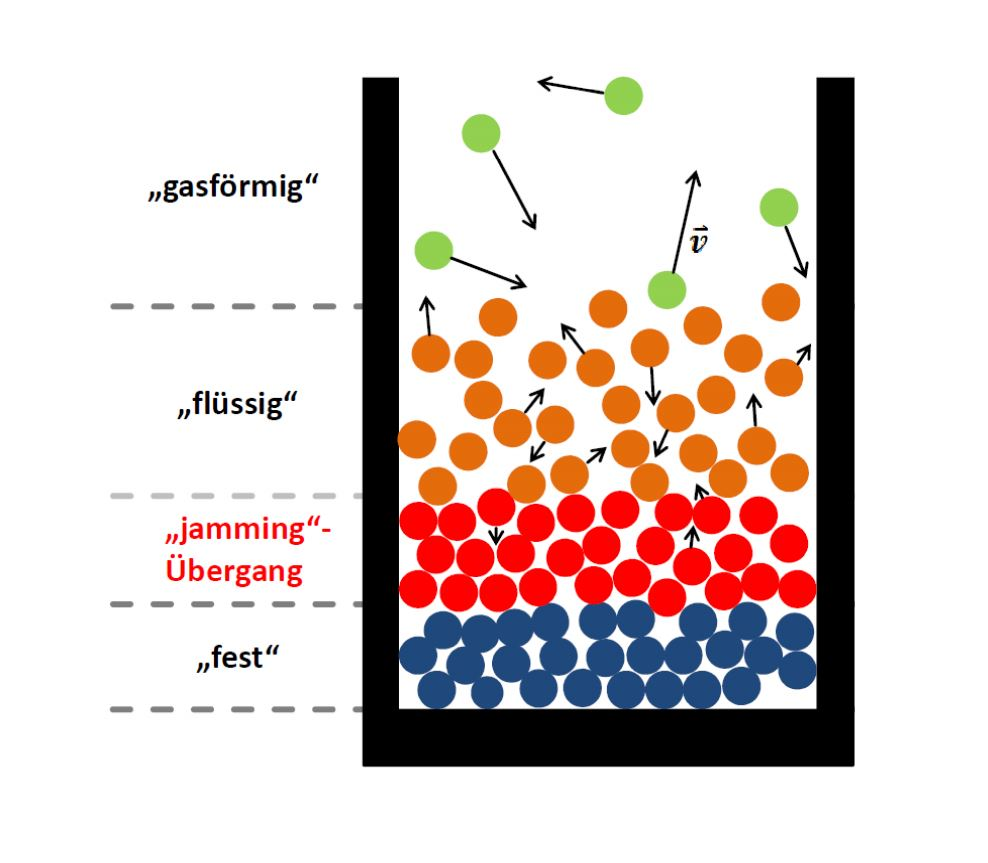
\includegraphics[scale=0.45]{Einleitung_1.jpg}
	\caption{Unterschiedliche Phasen eines Granulats}
\end{figure}	
\end{center}

Die in Abbildung 1.1 zu sehenden Phasen treten alle gleichzeitig während einer Anregung durch Vibration auf. \\
Im gasförmigen Zustand sind die Abstände der Partikel weit größer als der Partikeldurchmesser und die Partikel bewegen sich weitgehend unabhängig voneinander. \\
Der darunterliegende flüssige Zustand bietet bereits deutlich weniger Bewegungsfreiheit. Die mittlere freie Weglänge ist auf die Größenordnung der Partikel gesunken (fragen!). Man spricht auch von einem Glasübergang. \\
Charakteristisch für granulare Medien ist der \glqq jamming\grqq \ Übergang zwischen fest und flüssig. Hier ist keine Diffusion mehr möglich, die Partikel verbleiben also in ihrer Packungsposition und verklemmen mit ihrer Nachbarn. Bereits in diesem Zustand bilden sich sogenannte \glqq force chains\grqq \ heraus, über die die Kraftübertragung des Systems läuft. \\
Die \glqq force chains\grqq \ bilden sich im festen Zustand vollständig heraus und entstehen vor allem dadurch, das ein Teilchen deutlich mehr Nachbarn hat, als zu Stabilisation braucht. Da sich die Partikel amorph anordnen, verlaufen die \glqq force chains\grqq \ nicht homogen und isotrop, sondern willkürlich, was sich in einer unregelmäßigen Kraftverteilung ausdrückt.



\subsection{Ionisator}

Unter einem Ionisator versteht man ein Gerät, das ein Medium ionisiert und des dadurch elektrisch leitfähig macht. Je nach Bauweise und je nachdem wie das Gerät das Medium ionisiert, gibt es unterschiedliche Anwendungszwecke. \\
Ich beschränke mich hier auf einen Ionisator, der mittels eines starken elektrischen Feldes Luft ionisiert und unserem Anwendungszweck genügt. \\
Unser Ionisator besteht aus einem Netzteil, das $\SI{7}{\kilo V}$ Spannung erzeugt und einem Aufsatz, an dessen Ende ein elektrisches Feld zwischen der Metallspitze und dem äußeren Ring erzeugt wird.


Foto machen!!


\subsection{Flowcontroller}

Ein Flowcontroller ist ein Gerät mit dem man Flüsse gasförmiger oder flüssiger Medien kontrollieren kann. In der Regel kann ein Flowcontroller nur mit einem Aggregatzustand arbeiten und auch dort muss auf die verschiedenen Medien kalibriert werden, damit die angegeben Fehlergrenzen eingehalten werden. \\
Flowcontroller gibt es für viele verschiedene Flussraten, Genauigkeiten, Medien und Ansteuerungssysteme. Wie bei allen Produkten gilt auch hier das Prinzip, desto mehr Features, desto teurer der Controller. \\
Bei wissenschaftlichen Untersuchungen wie unserem Experiment kommt man um bestimmte Features nicht herum, da eine hohe Genauigkeit und präzises Ansteuern besonders wichtig sind. Dies wird im Abschnitt XXX genauer erläutert.



\section{Wissenschaftliche Fragestellung}

In der heutigen Zeit möchte man immer komplexere Metallteile am Stück formen, da dies, wegen weniger potentieller Bruchstellen, zu höherer Stabilität führt. Besonders ist man daran interessiert das jetzige Warmformgebungsverfahren bei hohlen Aluminiumprofilen auch für Stahlprofile nutzbar zu machen. \\
Dabei steht man vor der Herausforderung, das man bei den Temperaturen der Stahl Warmformgebung keine Ölmischung mehr nutzen kann, da sich diese entzünden würde. \\
Aus diesem Grund wählte man als Medium die Stoffklasse der granularen Medien aus. Diese bringen allerdings den Nachteil mit sich, das sie kompressiebel sind und die an einer Seite aufgebrachte Kraft sich nicht homogen und isotrop auf den Wänden verteilt. 
Man nimmt an, das die Art der Kraftverteilung durch drei Hauptparameter charakterisieren lässt. Zum einen ist das die Form der verwendeten Partikel, die Größe der Partikel und die Adhäsionskrafte der Partikel untereinander. \\
Diese drei Parameter kann man gesammelt betrachten, indem man die granularen Medien in einem Wirbelbett fluidisiert und misst ab wann die Medien in die flüssige Phase übergehen. Dadurch erreicht man eine Vergleichbarkeit der Medien untereinander und kann im Anschluss besser entscheiden welche Medien sich als Kraftüberträger eignen. \\


\section{Ziele der Arbeit}

In der Arbeit soll ein vorhandener Versuchsstand für quantitative Messungen optimiert werden und der Versuchsstand soll sowohl mit Luft als auch mit Wasser betrieben werden können. Im Praxisprojekt werden die Probleme des bisherigen Setups analysiert und eine entsprechende Lösung für das Medium Luft konstruiert. \\ 
Der Zeitraum der Bachelorarbeit beschäftigt sich mit der Konzeption in wie fern sich das Setup auf Wasserbetrieb umrüsten lässt und mit dessen Umsetzung. \\
Die Arbeit wurde dazu in folgende Arbeitspakete unterteilt:


\subsection{AP 1}

In einem ersten Schritt werden die Eckdaten den Projekts gesammelt und den Anforderungen zugeordnet. Zudem wird über die Materialwahl entschieden und eine Stückliste aller Kaufteile erstellt. Außerdem werden erste Lösungsansätze definiert, was wiederum in die Liste der Kaufteile einfließt.


\subsection{AP 2}

Die bisherige Elektronik liegt schutzlos und unübersichtlich neben dem Versuchsaufbau. Hier ist es erforderlich diese in sofern zu verpacken, das klar ist welche Anschlüsse für was gedacht sind und das ein eine einfache Transportierbarkeit gewährleistet ist.
Weiterhin muss ein A-D Wandler in die Schaltung integiert und angeschlossen werden.

\subsection{AP 3}

Zum Betrieb es Wirbelbettes ist ein Gaszustrom nötig, bei dem sich der momentane Gasstrom präzise zwischen $\SI{0}{\liter / \hour} - \SI{3000}{\liter / \hour}$ regeln und der dabei anliegende Druck messen lässt. Weiterhin soll eine Komponente zur Befeuchtung der Luft integriert werden, die variabel zu- und abgeschaltet werden kann. \\
Zudem muss soll das ganze System mechanisch stabil sein und transportabel sein. \\
Die Aufgabe besteht darin einen geeigneten Flowcontroller anzuschaffen, den Luftbefeuchter auszulegen und die Verrohrung entsprechend der Anforderungen zu wählen und umzusetzen.

\subsection{AP 4}

Das Wirbelbett ist die Hauptbaugruppe um die sich das Projekt dreht. In ihr befindet sich bei den Versuchen das granulare Medium und an ihr finden die optischen Messungen statt. \\
Hier besteht die Aufgabe in einer nahezu völligen Neukonstruktion, um das Bett für einen größeren Messraum nutzbar zu machen und auch einige neue Features hinzuzufügen.


\subsection{AP 5}

\subsection{AP 6}

\subsection{AP 7}



























\end{document}